\documentclass[12pt]{article}
\usepackage{../eplcrypto}
\usepackage{geometry} % see geometry.pdf on how to lay out the page. There's lots.
\geometry{a4paper} % or letter or a5paper or ... etc
% \geometry{landscape} % rotated page geometry
\usepackage[parfill]{parskip}
% See the ``Article customise'' template for come common customisations
\usepackage{amsmath}
\usepackage{graphicx}
\usepackage{amssymb}
\usepackage{algorithmic}
\usepackage{algorithm}

\usepackage{tikz}
\usetikzlibrary{calc,positioning}
\usepackage{amsfonts}
\usetikzlibrary{intersections}
\title{Slides06}

%%% BEGIN DOCUMENT
\begin{document}

\maketitle
\tableofcontents
\newpage

\section{Key Agreement}
\subsection{The Diffie-Hellman Protocol}
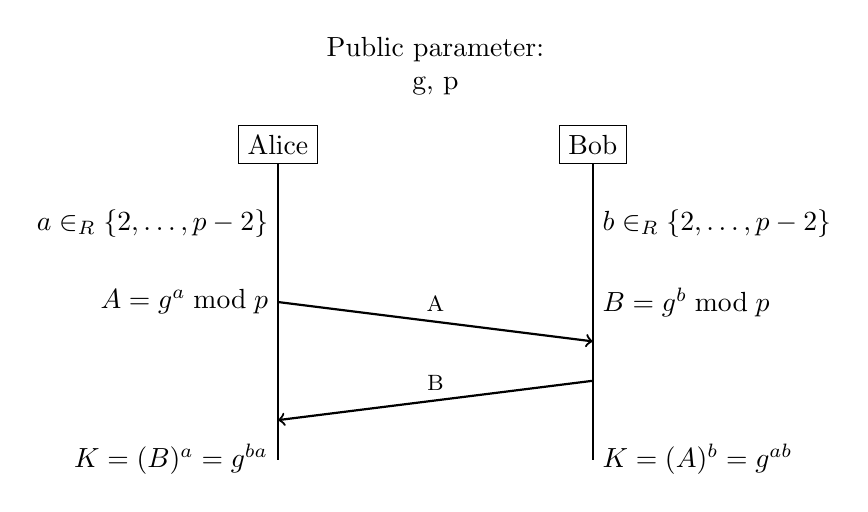
\begin{tikzpicture}
  % Public parameter:
  \node[draw=none,fill=none,align=center] (public) at (0,1) {Public parameter:\\g, p};
  
  % Alice
  \node[draw] (Alice) at (-2,0) {Alice}; 
  \draw[thick] (Alice) -- ++(0, -4);
    
  % Calculations of Alice
  \node[draw=none,fill=none,anchor=east] (asecret) at ($(Alice) + (0,-1)$) {$a \in_{R} \{2,\dots,p-2\}$};
  \node[draw=none,fill=none,anchor=east] (Apublic) at ($(Alice) + (0,-2)$) {$A = g^{a} \bmod{p}$};
  \node[draw=none,fill=none,anchor=east] (akey) at ($(Alice) + (0,-4)$) {$K = (B)^{a} = g^{ba}$};
    
  % Bob
  \node[draw] (Bob) at (2,0) {Bob}; 
  \draw[thick] (Bob) -- ++(0, -4);
   
  % Calculations of Bob
  \node[draw=none,fill=none,anchor=west] (bsecret) at ($(Bob) + (0,-1)$) {$b \in_{R} \{2,\dots,p-2\}$};
  \node[draw=none,fill=none,anchor=west] (Bpublic) at ($(Bob) + (0,-2)$) {$B = g^{b} \bmod{p}$};
  \node[draw=none,fill=none,anchor=west] (bkey) at ($(Bob) + (0,-4)$) {$K = (A)^{b} = g^{ab}$};
   
  % Messages
  \draw[->,thick] ($(Alice)+(0,-2)$) -- ($(Bob)+(0,-2.5)$) node [pos=0.5,above,font=\footnotesize] {A};
  \draw[->,thick] ($(Bob)+(0,-3)$) -- ($(Alice)+(0,-3.5)$) node [pos=0.5,above,font=\footnotesize] {B};
    
\end{tikzpicture}

\subsection{The Discrete Logarithm Problem}
\subsubsection{Experiment: $\Dlog(n)$}
\begin{enumerate}
\item Run $\G(1^n)$ to obtain ($\GG, q, g$) where $g$ generates the group $\GG$ of order $q$, with $|q|=n$
\item Choose $h \leftarrow \GG$
\item Set $x\leftarrow \A(\GG,q,g,h)$
\item $\Dlog(n)=1 \iff g^x=h$
\end{enumerate}

The discrete logarithm problem is hard relative to $\G$ if $\forall$ PPT $\A$, $\exists$ negl. $\negl$ s.t.:
\begin{equation*}
Pr[\Dlog(n)=1] \le \negl(n)
\end{equation*}
\newpage
\subsubsection{Generic algorithms for $\DLog$}
Given an instance $(\GG,q,g,h)$, how to find x?
\begin{enumerate}
\item Try all $x$ until $g^x=h$\\
Takes up to q attempts, and $|q|=128$ so looks good.
\item Baby-step, giant-step algorithm, with $s=\sqrt{q}$
	\begin{enumerate}
	\item Compute $g^s$ (takes $\O$($\sqrt{q}$) steps) 
	\item Compute $S=\{g^s, g^{2s}, \dots, g^{s^2}\}$  (takes $\O$($\sqrt{q}$) steps) 
	\item Search $i \in \{0,\dots,q\}$ s.t., if $g^i*h = g^{j*s} \in S$ (takes $\O$($\sqrt{q}$) steps) 
	\item return $x=js-i$
	\end{enumerate}
	Takes  $\O$($\sqrt{q}$) work, so $|q|=256$ looks good

\end{enumerate}



\section{Elliptic Curve Cryptography}
Groups defined on elliptic curves. They are harder to break, we can use shorter key sizes ($\ZZ_p$ 3072 bits is often compared to ECC 256 bits), and faster algorithms are possible with ECC.
\newpage
\subsection{How does it work?}
Groups are defined on the points of elliptic curves. Elliptic curves are defined by the equation:
\begin{equation*}
y^2 = x^3+Ax+B
\end{equation*}

\begin{figure}[ht]
    \centering
    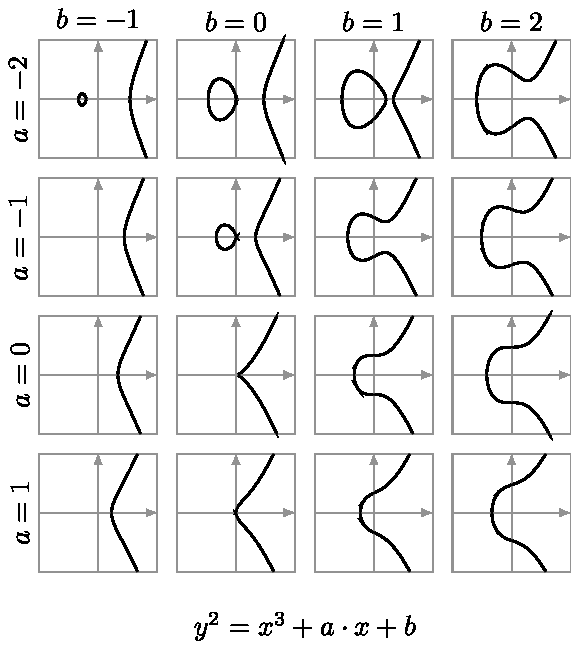
\includegraphics[width=8cm]{figures/ec_curves.png}
\end{figure}

In cryptography:
\begin{equation*}
y^2 = x^3+Ax+B \text{ mod }p
\end{equation*}
With constraints:
\begin{itemize}
\item $p>3$ is prime
\item $4A^3+27B^2 \neq 0 (\text{ mod }p)$ guarantees distinct roots, and avoids bad behaviour
\end{itemize}
Define:
\begin{itemize}
\item $E(\ZZ_p)\define \{(x,y) \in \ZZ_p \times \ZZ_p \text{ on the curve }\} \cup \O$
\item $\O$ is the point at infinity, can be imagined as the north pole which everywhere on earth has the meridians meeting at the north pole so $ (x, \infty) (\forall x)$
\end{itemize}
\newpage
\subsubsection{Example with $\ZZ_7$}
$f(x)=x^3-2x+2$ and so the curve would be $y^2 = f(x)$  mod 7\\
Each value of $x$ for which $f(x)$ is in $QR_7$ yields two points on the curve.\\
$QR_7 = \{0 (0^2),1 (1^2=6^2), 2 (3^2=4^2),4 (2^2=5^2)\}$
\begin{itemize}
\item f(0)=2 $\in QR_7$ (0,3) and (0,4)
\item f(1)=1 $\in QR_7$ (1,1) and (1,6)
\item f(2)=6 $\notin QR_7$
\item f(3)=2 $\in QR_7$ (3,3) and (3,4)
\item f(4)=2 $\in QR_7$ (4,3) and (4,4)
\item f(5)=5 $\notin QR_7$
\item f(6)=3 $\notin QR_7$
\end{itemize}
Which gives $|E(\ZZ_p)|=9$ (including $\O$)\\

Any line cutting an  EC twice cuts it in a 3rd point:
\begin{itemize}
\item A point is counted twice if line is tangent to EC
\item $\O$ counts too
\end{itemize}

\begin{figure}[ht]
    \centering
    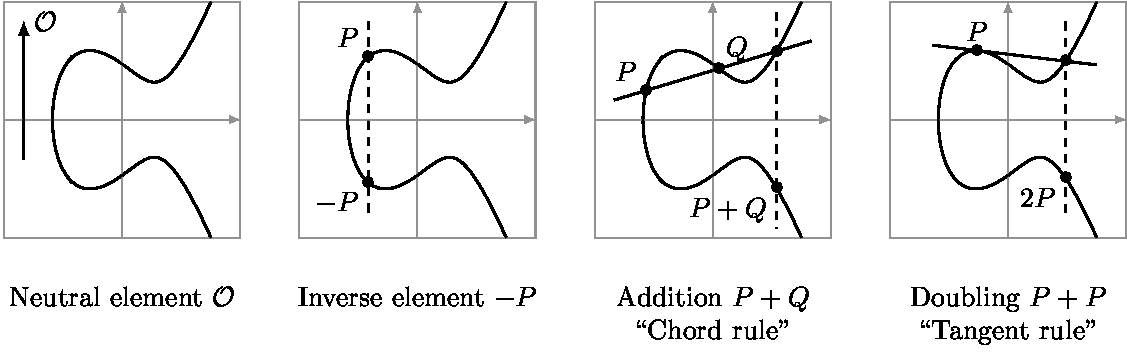
\includegraphics[width=14cm]{figures/ec_group_operations.png}
\end{figure}
\newpage
\section{Public Key Encryption}
A triple $\langle \Gen, \Enc, \Dec \rangle$ of PPT algorithms:
\begin{itemize}
\item $\Gen$ probabilistically selects $(pk,sk) \leftarrow \Gen(1^n)$
\item $\Enc$ provides $c\leftarrow \Enc_{pk}(m)$
\item $\Dec$ provides $m \define \Dec_{sk}(c)$
\end{itemize}
s.t., $\exists$ negl. $\negl$ : $\forall n$ $(pk,sk) \leftarrow \Gen(1^n)$, and $\forall m$:
\begin{equation*}
Pr[\Dec_{sk}(\Enc_{pk}(m))\neq m] < \negl(n)
\end{equation*}
Assumption: $|pk| \ge n$ and $|sk| \ge n$

\subsection{Experiment: $\PubKeav(n)$}
Given $\Pi \define \langle \Gen, \Enc, \Dec \rangle$ and PPT adversary $\A$.
\begin{enumerate}
\item Generate $(pk,sk) \leftarrow \Gen(1^n)$
\item $\A(pk)$ outputs $m_0, m_1$ of same length
\item Choose $b\leftarrow \bset$ and send $\Enc_{pk}(m_b)$ to $\A$
\item $\A$ outputs $b'$
\item Define $\PubKeav(n)\define 1 \iff b=b'$
\end{enumerate}
Difference with $\PrivKeav$ is that here $\A$ is given the $pk$ before choosing challenge messages.

$\Pi \define \langle \Gen, \Enc, \Dec \rangle$ has indistinguishable encryptions in the presence of eavesdroppers if $\forall$. PPT $\A$, $\exists$ negl. $\negl$:
\begin{equation*}
Pr[\PubKeav(n)=1] \le \frac12 + \negl(n)
\end{equation*}
\newpage

\subsection{Experiment: $\PubKcpa(n)$}
Given $\Pi \define \langle \Gen, \Enc, \Dec \rangle$ and PPT adversary $\A$.
\begin{enumerate}
\item Generate $(pk,sk) \leftarrow \Gen(1^n)$
\item $\A(pk)$ is given. oracle access to $\Enc_{pk}(\cdot)$ 
\item $\A(pk)$ outputs $m_0, m_1$ of same length
\item Choose $b\leftarrow \bset$ and send $\Enc_{pk}(m_b)$ to $\A$
\item $\A(pk)$ is again given. oracle access to $\Enc_{pk}(\cdot)$ 
\item $\A$ outputs $b'$
\item Define $\PubKcpa(n)\define 1 \iff b=b'$
\end{enumerate}
Difference with $\PrivKcpa$ is that here $\A$ is given the $pk$ before choosing challenge messages.

$\Pi \define \langle \Gen, \Enc, \Dec \rangle$ has indistinguishable encryptions in the presence of eavesdroppers if $\forall$. PPT $\A$, $\exists$ negl. $\negl$:
\begin{equation*}
Pr[\PubKcpa(n)=1] \le \frac12 + \negl(n)
\end{equation*}

\subsubsection*{What is the relationship between $\PubKeav$ and $\PubKcpa$?}
They are equivalent, since (pk) is known there is no need for an oracle.

\subsubsection*{Could we build a perfectly secure public key encryption scheme?}
No, since the adversary has the public key, he can take a challenge ciphertext c and encrypt the two challenge messages with all possible random coins until it gets c.

No, since the adversary has the public key, he can encrypt messages of his choice and search for the correct decryption key.
\newpage

\subsection{Experiment: $\PubKmult(n)$}
Given $\Pi \define \langle \Gen, \Enc, \Dec \rangle$ and PPT adversary $\A$.

\begin{enumerate}
	\item Generate $(pk,sk) \leftarrow \Gen(1^n)$
	\item $\A(pk)$ outputs $M_0 = (m_0^1,\dots,m_0^t), M_1=(m_1^1,\dots,m_1^t)$ 
	\item Choose $b\leftarrow \bset$ and send $(\Enc_{pk}(m_b^1),\dots,\Enc_{pk}(m_b^t))$ to $\A$
	\item $\A$ outputs $b'$
	\item Define $\PubKmult(n)\define 1 \iff b=b'$
\end{enumerate}

$\Pi \define \langle \Gen, \Enc, \Dec \rangle$ has indistinguishable multiple encryptions in the presence of eavesdroppers if $\forall$. PPT $\A$, $\exists$ negl. $\negl$:
\begin{equation*}
Pr[\PubKmult(n)=1] \le \frac12 + \negl(n)
\end{equation*}

\emph{If public-key encryption scheme $\Pi$ is CPA-secure, then it also has indistinguishable multiple encryptions}

\subsection{Experiment: $\PubKcca(n)$}
Given $\Pi \define \langle \Gen, \Enc, \Dec \rangle$ and PPT adversary $\A$.
\begin{enumerate}
\item Generate $(pk,sk) \leftarrow \Gen(1^n)$
\item $\A(pk)$ is given. oracle access to $\Enc_{pk}(\cdot)$ (it has pk so actually no need) and $\Dec_{pk}(\cdot)$
\item $\A(pk)$ outputs $m_0, m_1$ of same length
\item Choose $b\leftarrow \bset$ and send $\Enc_{pk}(m_b)$ to $\A$
\item $\A(pk)$ is again given. oracle access to $\Enc_{pk}(\cdot)$ and $\Dec_{pk}(\cdot)$
\item $\A$ outputs $b'$
\item Define $\PubKcca(n)\define 1 \iff b=b'$
\end{enumerate}
Difference with $\PrivKcca$ is that here $\A$ is given the $pk$ before choosing challenge messages.

$\Pi \define \langle \Gen, \Enc, \Dec \rangle$ has  indistinguishable encryptions under a chosen-ciphertext attack if $\forall$. PPT $\A$, $\exists$ negl. $\negl$:
\begin{equation*}
Pr[\PubKcca(n)=1] \le \frac12 + \negl(n)
\end{equation*}

\section{Elgamal Encryption}
A CPA-secure encryption scheme.\\
Idea: Use a session key to encrypt $m \in \GG$

\begin{tikzpicture}
  % Alice
  \node[draw] (Alice) at (-2,0) {Alice}; 
  \draw[thick] (Alice) -- ++(0, -10);
    
  % Calculations of Alice
  \node[draw=none,fill=none,anchor=east] (asecret) at ($(Alice) + (0,-1)$) {She runs $\G$: $(\GG,q,g) \leftarrow \G$};
  \node[draw=none,fill=none,anchor=east] (asecret) at ($(Alice) + (0,-2)$) {Picks $x\leftarrow \ZZ_q, \text{and sets }h\define g^x$};
  \node[draw=none,fill=none,anchor=east] (Apublic) at ($(Alice) + (0,-3)$) {$\langle pk,sk \rangle \define \langle(\GG,q,g,h),(\GG,q,g,x) \rangle$};
  \node[draw=none,fill=none,anchor=east] (akey) at ($(Alice) + (0,-7)$) {$m=\Dec_{sk}(\langle c_1,c_2 \rangle)\define \frac{c_2}{c_1^x}$};  
    
  % Bob
  \node[draw] (Bob) at (2,0) {Bob}; 
  \draw[thick] (Bob) -- ++(0, -10);
   
  % Calculations of Bob
  \node[draw=none,fill=none,anchor=west] (akey) at ($(Bob) + (0,-4)$) {He wants to encrypt: $m \in \GG$};
  \node[draw=none,fill=none,anchor=west] (akey) at ($(Bob) + (0,-5)$) {$y \leftarrow \ZZ_q$};
  \node[draw=none,fill=none,anchor=west] (akey) at ($(Bob) + (0,-6)$) {$\langle c_1,c_2 \rangle = \Enc_{pk}(m)\define \langle g^y,m\cdot h^y \rangle$};
 
  % Messages
  \draw[->,thick] ($(Alice)+(0,-3)$) -- ($(Bob)+(0,-3.5)$) node [pos=0.5,above,font=\footnotesize] {$\GG,q,g,h$};
  \draw[->,thick] ($(Bob)+(0,-6)$) -- ($(Alice)+(0,-6.5)$) node [pos=0.5,above,font=\footnotesize] {($\langle c_1,c_2 \rangle$)};
    
\end{tikzpicture}

\subsubsection*{Can we prove that Elgamal is CPA-secure based on the hardness of the $\DLog$ problem w.r.t $\G$? }
No: If I can compute the least significant bit of $h^y$ given $(g,h,g^y)$, then it is enough to break Elgamal, but not necessarily to solve $\DLog$. If you learn a few bits from $h^y$ then you learn few bits from the message which breaks CPA-security, however,  $\DLog$ asks you to compute $y$ so it is not really breaking  $\DLog$.

Therefore, we need something more than  $\DLog$ assumption: 
\begin{itemize}
\item It may be possible to compute $h^y$ without solving the  $\DLog$ (we do not know how, but we cannot exclude it)
\item We need $h^y$ to be completely unpredictable, else parts of m may be leaked.
\end{itemize}

This is also true for DH key agreement: The key $g^{xy}$ must be "as" a random key, not just a hard to compute value.
\newpage
\subsection{Computational Diffie-Hellman}
\subsubsection{Experiment: $\CDHn$}
\begin{enumerate}
\item Run $\G(1^n)$ to obtain $(\GG,q,g)$ where $<g>=\GG$ and $|\GG|=q$ with $|q|=n$
\item Choose $(x,y )\leftarrow \ZZ_q^2$
\item set $h\leftarrow \A(\GG,q,g,g^x,g^y)$
\item $\CDHn=1 \iff h=g^{x\cdot y}$ 
\end{enumerate}

The computational Diffie-Hellman problem is hard relative to $\G$\\
 if $\forall  \text{ PPT } \A$ $\exists \text{ negl. } \negl $ s.t.:
\begin{equation*}
Pr[\CDHn=1] \le \negl(n)
\end{equation*}

Observe:
\begin{itemize}
\item If $\Dlog(n)$ is easy then $\CDHn$ is easy
\item The converse is not true!
\end{itemize}


\subsection{Decisional Diffie-Hellman}
\subsubsection{Experiment: $\DDHn$}
\begin{enumerate}
\item Run $\G(1^n)$ to obtain $(\GG,q,g)$ where $<g>=\GG$ and $|\GG|=q$ with $|q|=n$
\item Choose $(x,y,z )\leftarrow \ZZ_q^3$
\item Pick $b \leftarrow \bset$, and set $h_1 \define g^{x\cdot y}$ and $h_0 \define g^z$ send $(g^x,g^y,h_b)$ to $\A$
\item $\A$ outputs $b'\leftarrow \A(\GG,q,g,(g^x,g^y,h_b))$
\item $\DDHn=1 \iff b=b' $
\end{enumerate}

No need to compute $g^{x\cdot y}$ or anything else, the $\A$ just decides if it sees $g^{x\cdot y}$ or $g^z$


The decisional Diffie-Hellman problem is hard relative to $\G$\\
 if $\forall  \text{ PPT } \A$ $\exists \text{ negl. } \negl $ s.t.:
\begin{equation*}
Pr[\DDHn=1] \le \frac12+ \negl(n)
\end{equation*}

Observe:
\begin{itemize}
\item If $\CDHn$ is easy then $\DDHn$ is easy
\item The converse is believed to be false
\end{itemize}
\subsection{Elgamal security reduction}
\begin{figure}[ht]
    \centering
    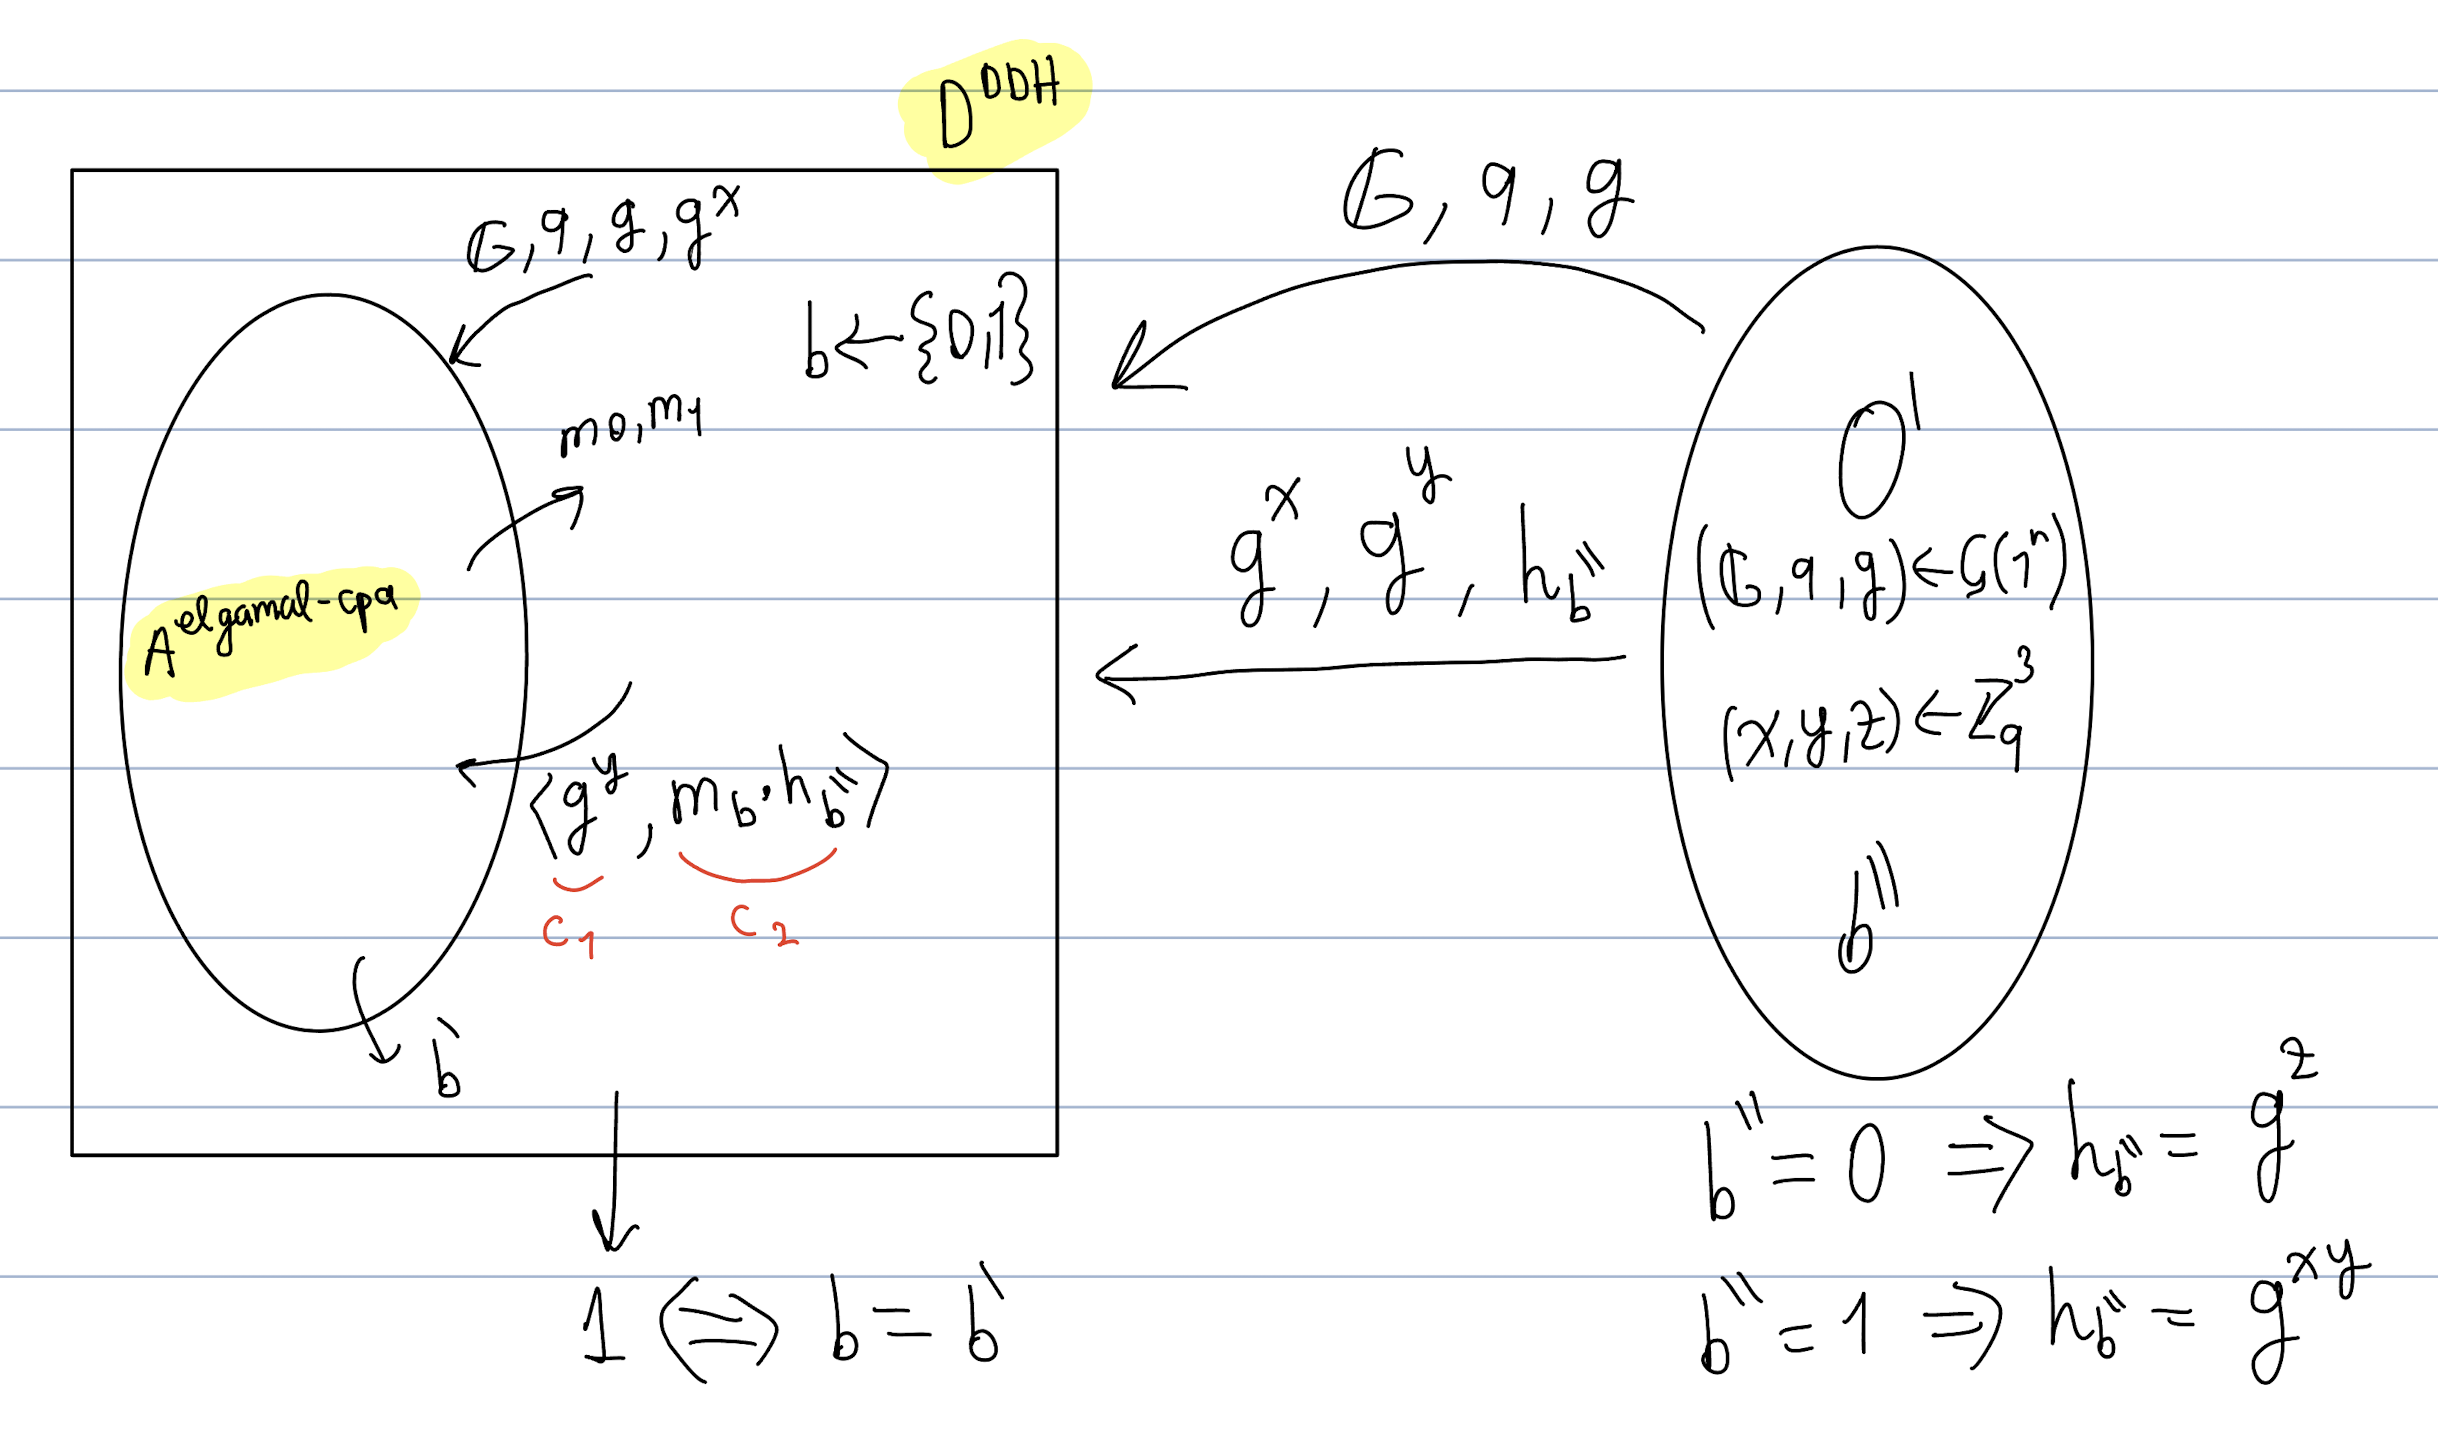
\includegraphics[width=16cm]{figures/f1.png}
    \caption{Elgamal security: $D^{DDH}$ using $A^{elgamal-cpa}$ as a subroutine to break DDH asumption}
\end{figure}
Observe:
\begin{itemize}
\item If $b''=0$, $Pr[D \text{ output } 1] = \frac12$ : idealized scheme\\
This corresponds to $m_b\cdot g^z$ being random in $\GG$ and it is the idealized scheme (step 1 of proof was to create an idealized scheme) so best case is that it flips a coin and outputs that.
\item If $b''=1$, $Pr[D \text{ output } 1] = \frac12 + \eta(n)$ : normal security game\\
Here, we have the normal game, we said that in the normal game $A^{elgamal-cpa}$ has the advantage of $\eta(n)$, we do not know it is negligible or not yet.
\end{itemize}
Now the point of the reduction is to see if $D^{DDH}$ can tell which world he is in (whether $b''=0$ or $b''=1$).
\newpage
Using the observations above we have:
\begin{equation*}
|Pr[D \text{ output } 1 \text{ when b''=1 }] - Pr[D \text{ output } 1 \text{ when b''=0 }]| = \eta(n)
\end{equation*}
Here we see that $D^{DDH}$ distinguishes which world he is in with the same advantage as $A^{elgamal-cpa}$. So this means that advantage of $A^{elgamal-cpa}$ $\eta(n)$ needs to be negligible.


\subsection{Elgamal can only encrypt short messages (one group element), panik} 
\begin{itemize}
\item Make many Elgamal ciphertexts $=>$ expensive
\item Solution: Derive a symmetric key from $g^{xy}$, and use it to encrypt the long message!
\end{itemize}

\subsubsection{DHIES/ECIES ($\approx$ ISE/IEC 18033-2) calm}
\begin{itemize}
\item $\Gen$ as in Elgamal, gives $\langle pk,sk \rangle \define \langle(\GG,q,g,h),(\GG,q,g,x) \rangle$
\item $\mathsf{ENC}_{pk}(m)$: pick $y\leftarrow \ZZ_q$, derive $k_e = H(h^y)$, return $(c_1,c_2)=\langle g^y, \Enc_{k_e}(m) \rangle$ with $\Enc$ part of an authenticated encryption scheme 
\item $\mathsf{DEC}_{sk}(c_1,c_2)$: Compute $k_e = H(c_1^x)$\\
return: $\Dec_{k_e}(c_2)$
\end{itemize}









\end{document}